\documentclass[tikz,border=20pt]{standalone}
\usepackage{amsmath}
\usetikzlibrary{positioning, arrows.meta, decorations.pathreplacing}

\begin{document}
	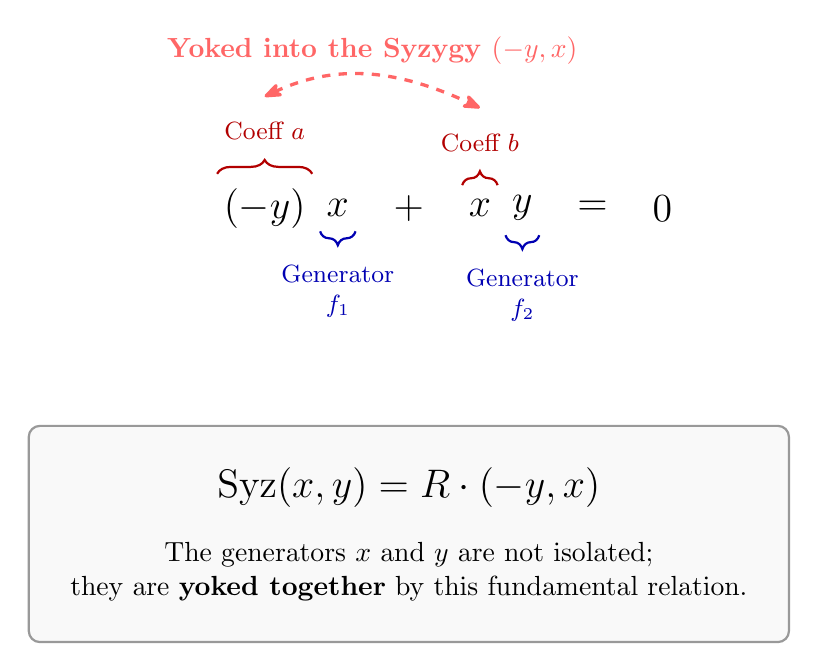
\begin{tikzpicture}[
		>={Stealth[round]}, thick,
		term/.style={font=\Large, inner sep=2pt}
		]
		
		% The main equation elements, spaced naturally
		\node[term] (t1) {$(-y)$};
		\node[term, right=0.1cm of t1] (t2) {$x$};
		\node[term, right=0.4cm of t2] (plus) {$+$};
		\node[term, right=0.4cm of plus] (t3) {$x$};
		\node[term, right=0.1cm of t3] (t4) {$y$};
		\node[term, right=0.4cm of t4] (eq) {$=$};
		\node[term, right=0.4cm of eq] (zero) {$0$};
		
		% Underbraces for Generators (Blue)
		\draw[decorate, decoration={brace, amplitude=5pt, mirror}, blue!70!black, thick] 
		([yshift=-0.1cm]t2.south west) -- ([yshift=-0.1cm]t2.south east) 
		node[midway, below=0.3cm, font=\small\color{blue!70!black}, align=center] {Generator\\$f_1$};
		
		\draw[decorate, decoration={brace, amplitude=5pt, mirror}, blue!70!black, thick] 
		([yshift=-0.1cm]t4.south west) -- ([yshift=-0.1cm]t4.south east) 
		node[midway, below=0.3cm, font=\small\color{blue!70!black}, align=center] {Generator\\$f_2$};
		
		% Overbraces for Syzygy parts (Red)
		\draw[decorate, decoration={brace, amplitude=5pt}, red!70!black, thick] 
		([yshift=0.1cm]t1.north west) -- ([yshift=0.1cm]t1.north east) 
		node[midway, above=0.3cm, font=\small\color{red!70!black}] (syz1) {Coeff $a$};
		
		\draw[decorate, decoration={brace, amplitude=5pt}, red!70!black, thick] 
		([yshift=0.1cm]t3.north west) -- ([yshift=0.1cm]t3.north east) 
		node[midway, above=0.3cm, font=\small\color{red!70!black}] (syz2) {Coeff $b$};
		
		% The "Yoke" connecting the coefficients
		\draw[<->, red!60, dashed, very thick] 
		([yshift=0.2cm]syz1.north) to[out=25, in=155] 
		node[midway, above, font=\bfseries\color{red!70!black}] {Yoked into the Syzygy $(-y, x)$} 
		([yshift=0.2cm]syz2.north);
		
		% Bottom conclusion box
		% We anchor it relative to the '+' sign to keep it centered under the equation
		\node[draw=black!40, rounded corners, fill=gray!5, inner sep=15pt, align=center, below=2.5cm of plus] (conclusion) {
			\Large $\operatorname{Syz}(x,y) = R \cdot (-y, x)$ \\[0.4cm]
			\normalsize The generators $x$ and $y$ are not isolated; \\
			\normalsize they are \textbf{yoked together} by this fundamental relation.
		};
		
	\end{tikzpicture}
\end{document}